    \documentclass[xcolor=x11names]{beamer}
%%%%%%%%%%%%%%%%%%%%%%%%%%%%%%%%%%%%%%%%%%%%%%%%%%%%%%%%%%%%
%%  This Beamer template was created by Cameron Bracken.
%%  Anyone can freely use or modify it for any purpose
%%  without attribution.
%%
%%  Last Modified by C. Bracken: January 9, 2009
%%
%%  The preamble, and maybe some modification of the Cameron Bracken's template is due to Attila Molnár.
%%
%%

%% General document
\usepackage[utf8]{inputenc}
\usepackage[T1]{fontenc}
\usepackage{graphicx}
\usepackage{tikz}
\usetikzlibrary{decorations.fractals}
\usetikzlibrary{decorations.text}
\usepgflibrary{arrows}
\usetikzlibrary{fadings}
\usetikzlibrary[decorations.pathmorphing]
\tikzfading[name=fade inside, inner color=transparent!70, outer color=transparent!70]
\usetikzlibrary{calc}
\usetikzlibrary{intersections}
\usetikzlibrary{shapes}
\usetikzlibrary{patterns}
\usefonttheme{serif}
\usepackage{amssymb} 			
\usepackage{amsmath}
\usepackage{ifthen}
\usepackage[normalem]{ulem}
\usepackage{mathrsfs}

%%%%%%%%%%%%%%%%%%%%%%%%%%%%%%%%%%%%%%%%%%%%%%%%%%%%%%%%%%%%%%%%%%%%%%%%%%%%%%%%%%%%
%% Beamer Layout %%%%%%%%%%%%%%%%%%%%%%%%%%%%%%%%%%
\useoutertheme[subsection=false,shadow]{miniframes}
\useinnertheme{default}
\usefonttheme{serif}
%\usepackage{txfonts} %Hook for strict implication!
\DeclareSymbolFont{symbolsC}{U}{txsyc}{m}{n}
\DeclareMathSymbol{\strictif}{\mathrel}{symbolsC}{74}
\DeclareMathSymbol{\boxright}{\mathrel}{symbolsC}{128}
\usepackage{palatino}
%\usepackage[uppercase=upright,charter]{mathdesign}

\setbeamerfont{title like}{shape=\scshape}
\setbeamerfont{frametitle}{shape=\scshape}


\setbeamercolor*{lower separation line head}{bg=white!40!DeepSkyBlue3}
\setbeamercolor*{normal text}{fg=black,bg=white}
\setbeamercolor*{alerted text}{fg=red}
\setbeamercolor*{example text}{fg=black}
\setbeamercolor*{structure}{fg=black}

\setbeamercolor*{palette tertiary}{fg=black,bg=white!90!DeepSkyBlue3}
\setbeamercolor*{palette quaternary}{fg=black,bg=black!10}

%\setbeamercolor{block body alerted}{bg=normal text.bg!90!DeepSkyBlue4}
\setbeamercolor{block body}{bg=normal text.bg!95!DeepSkyBlue3}
%\setbeamercolor{block body example}{bg=normal text.bg!90!DeepSkyBlue4}
%\setbeamercolor{block title alerted}{use={normal text,alerted text},fg=alerted text.fg!75!normal text.fg,bg=normal text.bg!90!DeepSkyBlue4}
\setbeamercolor{block title}{bg=normal text.bg!70!DeepSkyBlue3}
%\setbeamercolor{block title example}{use={normal text,example text},fg=example text.fg!75!normal text.fg,bg=normal text.bg!75!DeepSkyBlue4}

\setbeamertemplate{blocks}[rounded][shadow=true]
%\setbeamertemplate{background canvas}[vertical shading][bottom=white,top=structure.fg!25]
%\setbeamertemplate{sidebar canvas left}[horizontal shading][left=white!40!black,right=black]
\setbeamertemplate{itemize items}[circle]
\setbeamercolor*{itemize item}{fg=DeepSkyBlue3}
\setbeamercolor*{itemize subitem}{fg=DeepSkyBlue3}
\setbeamercolor*{itemize subsubitem}{fg=DeepSkyBlue3}
\setbeamertemplate{enumerate items}[circle]
%\setbeamercolor{item projected}{bg=DeepSkyBlue3,fg=black}
\setbeamercolor{item projected}{bg=white,fg=DeepSkyBlue3}
\setbeamercolor*{enumerate item}{fg=DeepSkyBlue3}
\setbeamercolor*{enumerate subitem}{fg=DeepSkyBlue3}
\setbeamercolor*{enumerate subsubitem}{fg=DeepSkyBlue3}

%%%%%%%%%%%%%%%%%%%%%%%%%%%%%%%%%%%%%%%%%%%%%%%%%%


%%%%%%%%%%%%%%%%%%%%%%%%%%%%%%%%%%%%%%%%%%%%%%%%%%%%%%%%%%%%%%%%%%%%%%%%%%%%%%%%%%%%

\newenvironment{defi}[1][]{\begin{block}{\footnotesize \textsc{Definition} \ifthenelse{\equal{#1}{}}{}{\, (#1)}}}{\end{block}}
\newenvironment{prop}[1][]{\begin{block}{\footnotesize \textsc{Proposition} \ifthenelse{\equal{#1}{}}{}{\, (\textsc{#1})}}}{\end{block}}
\newenvironment{lemm}[1][]{\begin{block}{\footnotesize \textsc{Lemma} \ifthenelse{\equal{#1}{}}{}{\, (\textsc{#1})}}}{\end{block}}
\newenvironment{idea}[1][]{\begin{block}{\footnotesize \textsc{Idea} \ifthenelse{\equal{#1}{}}{}{\, (\textsc{#1})}}}{\end{block}}
\newenvironment{rema}[1][]{\begin{block}{\footnotesize \textsc{Remark} \ifthenelse{\equal{#1}{}}{}{\, (\textsc{#1})}}}{\end{block}}
\newenvironment{coro}[1][]{\begin{block}{\footnotesize \textsc{Corollary} \ifthenelse{\equal{#1}{}}{}{\, (\textsc{#1})}}}{\end{block}}
\newenvironment{tete}[1][]{\begin{block}{\footnotesize \textsc{Theorem} \ifthenelse{\equal{#1}{}}{}{\, (\textsc{#1})}}}{\end{block}}
\newenvironment{claim}[1][]{\begin{block}{Claim \ifthenelse{\equal{#1}{}}{}{\, (\textsc{#1})}}}{\end{block}}
%\newenvironment{lemma}[1][]{\begin{block}{Lemma \ifthenelse{\equal{#1}{}}{}{\, (\textsc{#1})}}}{\end{block}}
\newenvironment{question}[1][]{\begin{block}{Question \ifthenelse{\equal{#1}{}}{}{\, (\textsc{#1})}}}{\end{block}}
\newenvironment{rem}[1][]{\begin{block}{Remark \ifthenelse{\equal{#1}{}}{}{\, (\textsc{#1})}}}{\end{block}}
\newenvironment{homework}[1][]{\begin{block}{Homework \ifthenelse{\equal{#1}{}}{}{\, (\textsc{#1})}}}{\end{block}}
\newenvironment{proo}[1][]{\begin{block}{\footnotesize \textsc{Proof} \ifthenelse{\equal{#1}{}}{}{\, (\textsc{#1})}}}{\end{block}}

%%%%%%%%%%%%%%%%%%%%%
%% To evade unnecessary circles, mainly for \cimdia
%%%%%%%%%%%%%%%%%%%%%

\makeatletter
\let\beamer@writeslidentry@miniframeson=\beamer@writeslidentry
\def\beamer@writeslidentry@miniframesoff{%
  \expandafter\beamer@ifempty\expandafter{\beamer@framestartpage}{}% does not happen normally
  {%else
    % removed \addtocontents commands
    \clearpage\beamer@notesactions%
  }
}
\newcommand*{\miniframeson}{\let\beamer@writeslidentry=\beamer@writeslidentry@miniframeson}
\newcommand*{\miniframesoff}{\let\beamer@writeslidentry=\beamer@writeslidentry@miniframesoff}
\makeatother

%%%%%%%%%%%%%%%%%%%%%%%%%%%%%
%%%%%%%%%%%%% END %%%%%%%%%%%
%%%%%%%%%%%%%%%%%%%%%%%%%%%%%


%%%% Formatting Commands

\newcommand{\cimdia}[1] {\miniframesoff \begin{frame}\begin{center}\huge \begin{tabular}{c}#1\end{tabular}\end{center}\end{frame}\miniframeson}
\newcommand{\szakasz}[2][]{\section{#1}\subsection{}\cimdia{#2}}
\newcommand{\bluebullet}{\textcolor{DeepSkyBlue3}{\quad $\bullet$} \,\,}

\newenvironment{frame*}[1][]{\miniframesoff \begin{frame} #1}{\end{frame}\miniframeson}

  % for admissible intersections
  \newcommand{\bigsqcap}{\rotatebox[origin=c]{180}{$\bigsqcup$}}

\newcommand{\felkorvonal}[2]{\draw[rounded corners=0] (180+#1:.25*#2 cm) arc (180+#1:360+#1:.25*#2 cm)--cycle;}
\newcommand{\pecset}[2]{\begin{tikzpicture}[remember picture,overlay]
\node [ draw=red, rectangle, rounded corners=5mm, inner sep=1mm, ultra thick, fill=white, fill opacity=.8, rotate=30, scale=#1, text opacity=0.7] at (current page.center) {#2};\end{tikzpicture}}

\newcommand{\felirat}[7][]{\begin{tikzpicture}[remember picture,overlay]
\node [draw=DeepSkyBlue3, rectangle, rounded corners=#3 mm, inner sep=#2mm, ultra thick, fill=white, fill opacity=.8, scale=#4, text opacity=1,#1]
at ([xshift=#5 cm, yshift=#6 cm]current page.center) {#7};
\end{tikzpicture}}

\newcommand{\hazi}[6]{\begin{tikzpicture}[remember picture,overlay]
\node [ draw=Coral1,
        rectangle,
        rounded corners=#2 mm,
        inner sep=#1mm,
        ultra thick,
        fill=white,
        fill opacity=.8,
        rotate=0,
        scale=#3,
        text opacity=1]
        at ([xshift=#4 cm, yshift=#5 cm]current page.center)
        {#6};
\end{tikzpicture}}

\newcommand{\underconstruction}[1]{\begin{tikzpicture}[remember picture,overlay]
\node [rectangle, rounded corners=5mm, inner sep=1mm, rotate=30, scale=#1, text opacity=0.4]at (current page.center){\textsc{\textcolor{orange}{\begin{tabular}{c}under \\construction\end{tabular}}}};
\end{tikzpicture}}

\newcommand{\dzsa}[1]{\textsc{\underline{#1}}:}
\newcommand{\axiom}[1]{\bemph{(\mathrm{#1})}}



% Emphasizing:
\definecolor{barna}{rgb}{0.5,0.2,0.1}
\newcommand{\bemph}[1] {{\color{DeepSkyBlue3}{#1}}}
\newcommand{\kemph}[1] {{\color{blue}{#1}}}
\newcommand{\cemph}[1]{\textcolor{red}{#1}}
\newcommand{\zemph}[1] {{\color{Green2}{#1}}}
\newcommand{\yemph}[1] {{\color{Orange1}{#1}}}
%\renewcommand{\emph}[1]{\textbf{#1}}

\newcommand{\FD}{\mathbf F}
\newcommand{\FB}{\mathbf G}
\newcommand{\PD}{\mathbf P}
\newcommand{\PB}{\mathbf H}
\newcommand{\GB}{\mathbf A}
\newcommand{\GD}{\mathbf E}

\newcommand{\Pmodels}{\mathrel{\models \hspace{-1.8ex} \raisebox{1.1ex}{\scalebox{.5}{$\mathrm{\bemph{P}}$}} }\,}
\newcommand{\Omodels}{\mathrel{\models \hspace{-1.8ex} \raisebox{1.1ex}{\scalebox{.5}{$\mathrm{\bemph{O}}$}} }\,}
\newcommand{\Kmodels}{\mathrel{\models \hspace{-1.8ex} \raisebox{1.1ex}{\scalebox{.5}{$\mathrm{\bemph{K}}$}} }\,}
\newcommand{\Bmodels}{\mathrel{\models \hspace{-1.8ex} \raisebox{1.1ex}{\scalebox{.5}{$\mathrm{\bemph{B}}$}} }\,}
\newcommand{\tru}{\textup{true}}
\newcommand{\fal}{\textup{false}}
\newcommand{\und}{\textup{undefined}}


\newcommand{\FDDot}{\underline{\mathbf F}}
\newcommand{\FBDot}{\underline{\mathbf G}}
\newcommand{\PDDot}{\underline{\mathbf P}}
\newcommand{\PBDot}{\underline{\mathbf H}}

\newcommand{\CFD}{\mathbf F^c}
\newcommand{\CFB}{\mathbf G^c}
\newcommand{\CPD}{\mathbf P^c}
\newcommand{\CPB}{\mathbf H^c}

\newcommand{\CFDDot}{\underline{\mathbf F^c}}
\newcommand{\CFBDot}{\underline{\mathbf G^c}}
\newcommand{\CPDDot}{\underline{\mathbf P^c}}
\newcommand{\CPBDot}{\underline{\mathbf H^c}}

\renewcommand{\Diamond}{\scalebox{.9}{\raisebox{-.4ex}{\rotatebox{45}{$\Box$}}}}

%causal
\newcommand{\past}{\succ}
\newcommand{\pasteq}{\succeq}
\newcommand{\future}{\prec}
\newcommand{\futureeq}{\preceq}
%lightlike
\newcommand{\llpast}{\nwarrow}
\newcommand{\llpasteq}{\underline\nwarrow}
\newcommand{\llfuture}{\nearrow}
\newcommand{\llfutureeq}{\mathop{\underline\nearrow}}
%timelike
\newcommand{\tlpast}{\gg}
\newcommand{\tlpasteq}{\underline \gg}
\newcommand{\tlfuture}{\ll}
\newcommand{\tlfutureeq}{\underline \ll}

\newcommand{\egyuttjar}{\mathop{\uparrow \uparrow}}
\newcommand{\Between}{\mathrm{B}}
\newcommand{\EqDist}{\equiv}
\newcommand{\ISCM}{\uparrow\equiv\uparrow}

 \newcommand{\vonal} [1][.2]{\hspace{#1cm} | \hspace{#1cm}}

 \newcommand{\lrule}[3][c]{\begin{array}{#1} #2  \\  \hline #3 \end{array}}
 \newcommand{\dlrule}[3][c]{\begin{array}{#1} #2  \\  \hline\hline #3 \end{array}}
 \newcommand{\dual}{\delta}

 \newcommand{\mono}{\rightarrowtail}
 \newcommand{\epi}{\twoheadrightarrow}
 \newcommand{\iso}{\rightarrowtail \!\!\!\!\! \rightarrow}

 \newcommand{\defegy}[1][.1]{\hspace{#1cm}\overset{\textup{\tiny def}}{=}\hspace{#1cm}}
 \newcommand{\defpont}[1][.1]{\hspace{#1cm}\overset{\textup{\tiny def}}{:}\hspace{#1cm}}
 \newcommand{\defekv}[1][.1]{\hspace{#1cm}\overset{\textup{\tiny def}}{ \Leftrightarrow }\hspace{#1cm}}
 \newcommand{\lthen}{\rightarrow}
 \newcommand{\liff}{\leftrightarrow}
 \newcommand{\forallin}[2]{(\forall #1 \in #2)}
 \newcommand{\existsin}[2]{(\exists #1 \in #2)}
 \newcommand{\nexistsin}[2]{(\nexists #1 \in #2)}
 \newcommand{\forallp}[1]{(\forall #1)}
 \newcommand{\existsp}[1]{(\exists #1)}

 \newcommand{\points}[1][0]{\hspace{#1ex}\hspace{-.5ex}:\hspace{-.5ex}\hspace{#1ex}}
 \newcommand{\Points}{\mathrm{P}}
 \newcommand{\Pointsf}{\mathrm{p}}
 \newcommand{\Ex}{\mathrm{E}}

\newcommand{\wline}[1]{\mathrm{wline}_{#1}}

\newcommand{\magyi}[1]{\textup{\bemph{\tiny #1}}}
\newcommand{\magyarazat}[2]{\overset{\substack{\textup{#2}\\ \downarrow}}{#1}}
\newcommand{\wintension}[3][]{{[}\hspace{-.46mm}{[} {#3}{]}\hspace{-.46mm}{]}^{\mathfrak{#1}}_{#2}}
\newcommand{\canintension}[2][]{{[}\hspace{-.46mm}{[} {#2}{]}\hspace{-.46mm}{]}_{\mathrm{#1}}}
\newcommand{\intension}[2][]{{[}\hspace{-.46mm}{[} {#2}{]}\hspace{-.46mm}{]}^{\mathfrak{#1}}}

\newcommand{\theory}[2][]{\mathrm{th}_{\mathfrak{#1}}(#2)}

\newcommand{\seenby}{\reflectbox {$R$}}
\newcommand{\derives}[1][]{\vdash_{\mathrm{#1}}}


\newcommand{\PBTemplate}[1]{{#1} \overrightarrow {\PB}}
\newcommand{\FBTemplate}[1]{{#1} \overrightarrow {\FB}}
\newcommand{\BoxTemplate}[1]{{#1} \overrightarrow {\Box}}
\newcommand{\PDTemplate}[1]{{#1} \widehat {\PD}}
\newcommand{\FDTemplate}[1]{{#1} \widehat {\FD}}
%\newcommand{\DiamondTemplate}[1]{#1\hspace{-.2ex} \mathop{\Diamond\hspace{-1.35ex} \raisebox{.4ex}{\scalebox{.5}{$\land$}}}\,}

%%%%%%%%%%%%%%%%%%%%%%%%%%%%%%%%%%%%%%%%%%%%%%%%%%%%%%
\newenvironment{tomb}[2][.1]{\arraycolsep=#1cm\begin{array}{#2}}{\end{array}}

\beamertemplatenavigationsymbolsempty


\author{Attila Moln\'ar}
\date{2014. March 21.}
\title{Test}
\institute{ELTE}
\begin{document}
\footnotesize


\szakasz[Ockhamist axioms]{Ockhamist axioms}

\begin{frame}[t]
\frametitle{$\mathbf O:$% \defegy \mathbf{K4.3}_{\FD, \PD} + \mathbf{S5}_{\scalebox{.7}{\Diamond}}$} %= \mathbf K.3_{\FD,\PD} + \mathbf S5_\Diamond + (IRR)+(UPP)+(WDC1)+(WDC2)+(MB)$}
%\framesubtitle{
%Logic of Kamp-frames and 
Ockhamist bundled trees}
\scriptsize
\begin{minipage}[t]{5.78cm}
$\mathbf{PC}$: {Classical logic}
\begin{itemize}
\item[(PC1)] $\varphi \lthen .\psi \lthen \varphi$
\item[(PC2)] $\varphi\lthen (\psi \lthen \chi) \lthen\!\!. (\varphi \lthen \psi) \lthen\!\! . \varphi \lthen \chi$
\item[(PC3)] $\varphi \lthen \psi \lthen .\lnot \psi \lthen \lnot \varphi$
\item[(MP)] $\lrule {\varphi , \; \varphi \lthen \psi}{\psi}$
\end{itemize}
\pause %%%%%%%%%%%%%%%%%%%%%% PAUSE %%%%%%%%%%%%%%%%%%%%%%%
\bemph{\hrule}
\smallskip

$\mathbf{K4.3_{\FD, \PD}}$: {Temporal logic of linear frames}
\begin{itemize}
\item[(A)] $(\FB\varphi \land \FB \psi )\lthen \FB(\varphi \land \psi )$,\quad  $(\PB\varphi \land \PB \psi )\lthen \PB(\varphi \land \psi )$
\item[(Lem)] $\lrule{\varphi\lthen \psi}{\PB\varphi \lthen \PB\psi}$, \quad $\lrule{\varphi\lthen \psi}{\FB\varphi \lthen \FB\psi}$
\item[(C)] $\PD\FB\varphi \lthen \varphi $, \quad  $\FD\PB\varphi \lthen \varphi$
\item[(4)] $\FB\varphi\lthen \FB\FB\varphi$
\item[(.3)] $\PB(\PBDot \varphi\lthen \psi ) \lor \PB(\PBDot \psi\lthen \varphi )$, \quad $\FB(\FBDot \varphi\lthen \psi ) \lor \FB(\FBDot \psi\lthen \varphi )$
\end{itemize}
\pause %%%%%%%%%%%%%%%%%%%%%% PAUSE %%%%%%%%%%%%%%%%%%%%%%%
\bemph{\hrule}
\smallskip
Irreflexivity rule:
\begin{itemize}
\item[(IRR)] $\lrule{(p\land \mathbf H \lnot p) \lthen \varphi}{\varphi}$  \textup{\tiny where $p$ does not occur in $\varphi$}
\end{itemize}
\end{minipage}\quad
\begin{minipage}[t]{4.7cm}
\pause
$\mathbf{S5}_{\Diamond}$: {Alethic
logic of equiv. relations}
\begin{itemize}
\item[(A)] $(\Box\varphi \land \Box \psi )\lthen \Box(\varphi \land \psi )$
\item[(Lem)] $\lrule{\varphi\lthen \psi}{\Box\varphi \lthen \Box\psi}$
\item[(T)] $\Box \varphi \lthen \varphi$
\item[(4)] $\Box \varphi\lthen \Box \Box \varphi$
\item[(B)] $\Diamond \Box \varphi \lthen \varphi$
\end{itemize}
\pause %%%%%%%%%%%%%%%%%%%%%% PAUSE %%%%%%%%%%%%%%%%%%%%%%%
\bemph{\hrule}
\smallskip
Full-blooded Ockhamist axioms
\begin{itemize}
\item[(UPP)] $ \varphi \lthen \Box \varphi $ {\tiny where $\FD $ does not occur in $\varphi$}.\\ \hfill \magyi{unpreventability of past}
\item[(WDC)] $ \varphi\lthen \FB \Box \PD \Diamond \varphi$ \\ \hfill \magyi{weak diagram completion}
\item[(WDC+)]$ (p \land \PB \lnot p \land \Box \varphi) \lthen $ \\ \hfill $\lthen \FB \Box \PB ((p \land \PB \lnot p) \lthen \varphi)$
\item[(MB)]  $ \FB \bot \lthen \Box \FB \bot $ \hfill \magyi{maximality of branches}
\end{itemize}
\end{minipage}
\end{frame}
%%%%%%%%%%%%%%%%%%%%%%%%%%%%%%%%%%%%%%%%%%%%%%%%%%%%%%%%%%%%%%%%%%%%%%%%%%
\begin{frame}[t]
	\frametitle{Plan}
\footnotesize
\begin{enumerate}
\item We construct an \cemph{irreflexive} submodel $\mathfrak M_K^-$ of the canonical Kamp model $\mathfrak M_K$. We will prove that we can use that model to prove a completeness proof, i.e., we prove a
\begin{enumerate}\footnotesize
\item Lindenbaum-type lemma
\item Existence Lemma
\item Truth Lemma
\item The Canonical model is \cemph{almost} a Kamp model -- canonicity proofs for all property except the maximality of histories.
\end{enumerate}
\item We transform $\mathfrak M_K^-$ into an $\mathrm M(\mathfrak M_K^-)$ in which the histories are maximal.
\item We prove that $\mathfrak M_K^-$ is a zig-zag image of $\mathrm M(\mathfrak M_K^-)$. 
\\ \magyi{We can conclude a completeness theorem for Kamp semantics}
\item We construct a bundled tree model from $\mathfrak M_K$ which satisfy the same formulas as $\mathrm M(\mathfrak M_K^-)$.
\\ \magyi{We can conclude a completeness theorem for bundled tree semantics}\end{enumerate}
\end{frame}
%%%%%%%%%%%%%%%%%%%%%%%%%%%%%%%%%%%%%%%%%%%%%%%%%%%%%%%%%%%%%%%%%%%%%%%%%%
\szakasz[Irreflexivity]{Irreflexivity}
\begin{frame}[t]
	\frametitle{Irreflexivity again}
\scriptsize
A canonical model usually has loops, and since we can not define irreflexivity, we can not remove those loops by adding new axioms to the logic. Previous solutions were:
\begin{itemize}
\item[Unraveling] In case of K4, We \emph{unravelled} the canonical model into an irreflexive, intransitive, antisymmetric tree, and then we took the transitive closure of the alternative relation, so we got an SPO. And since the canonical model of K4 is a zig-zag-image of this SPO, they satisfy the same formulas, so we can use it to prove completeness.
\pause
\item[Bulldozing] In case of K4.3, We \emph{bulldozed} the canonical model's clusters (so the loops as well) into backward and forward infinite lines. Since .3 formulas were canonical for non-branching, we got an STO. And since the canonical model of K4.3 is a zig-zag-image of this STO, they satisfy the same formulas, so we can use it to prove completeness.
\pause
\item[IRR-rule] The philosophy of the previous ideas was that the canonical model is too compressed: They unravelled it, or replaced the clusters with infinite routes. This idea is that we can \cemph{sort out the worlds that have loops} without losing the useful properties of canonical model. So this solution is about to make the canonical model \cemph{smaller}, not larger.
\end{itemize}


\end{frame}

%%%%%%%%%%%%%%%%%%%%%%%%%%%%%%%%%%%%%%%%%%%%%%%%%%%%%%%%%%%%%%%%%%%%%%%%%%
\begin{frame}[t]
	\frametitle{IRR-theories}
\scriptsize

Let us consider a loop as a \cemph{sin}.

\bigskip

A canonical world (m.c.s.) $\Gamma$ \cemph{can prove its innocence easily} iff
\[p \land \mathbf H \lnot p \in \Gamma \textup{ for some $p\in \mathrm {At}$.}\]
A canonical world (m.c.s.) $\Gamma$ \cemph{is in the company of easily provable innocents} iff
\[\lrule[l] {\mathrm{M}_1 (\varphi_1 \land \mathrm{M}_2 (\varphi_2 \land \dots \land \mathrm{M}_{n-1}(\varphi_{n-1}\land \mathrm M_n\varphi_n )\dots ))\in \Gamma}
         {
         \textup{There is a $p\in \mathrm{At}$ not occurring in $\varphi_1, \dots , \varphi_n$, s.t.}
         \\ \mathrm{M}_1 (\varphi_1 \land \mathrm{M}_2 (\varphi_2 \land \dots \land \mathrm{M}_{n-1}(\varphi_{n-1}\land \mathrm M_n(\varphi_n\land p \land \mathbf H \lnot p) )\dots ))\in \Gamma}\]
where $\mathrm{M}_i\in \{\Diamond, \FD, \PD\}$ for all $i\leq n$. 

\bigskip
Consider $\varphi_1, \dots, \varphi_n$ as tags of accessible worlds. The nested occurrences of ``$\mathrm{M}_i (\varphi_i \land$'' represents a search of the neighbour worlds where temporarily we tag every world with a formula that occurs there. The $i$-th step is made by $\mathrm{M}_i$, and the tag of that world is $\varphi_i$.

\vspace{-2em}
\[\scriptsize
\usetikzlibrary[shapes.arrows]
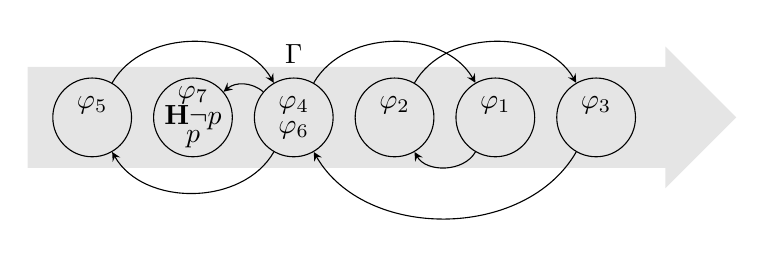
\begin{tikzpicture}[>=stealth, scale=.8,
world/.style={minimum size=1cm, draw=black, circle},
intension/.style={fill=black, fill opacity=.1},
altrel/.style={->},
bejaras/.style={blue}]

%%%%%%%%%%% SETTINGS %%%%%%%%%%%%%%%
\pgfmathsetmacro{\HorDist}{1.6}
\pgfmathtruncatemacro{\Darab}{6}
\pgfmathtruncatemacro{\EdgeAngle}{60}

%%%%%%%%%%% SZÁMOLANDÓK %%%%%%%%%%%%%%%
\pgfmathtruncatemacro{\nyilhossz}{\Darab+3}

\foreach \i in {1,2, ..., \Darab}
{\node[world](v\i) at (\HorDist*\i,0){};}

\node[single arrow,
fill=black,
fill opacity=.1,
single arrow head extend=.05cm,
minimum height=\nyilhossz cm,
minimum width=1.8cm,
single arrow head indent=0cm] at (1+.5*\HorDist*\Darab,0){};

\node at (3*\HorDist ,1) {$\Gamma$};

\draw[->] (v3) edge[in = 180-\EdgeAngle, out=\EdgeAngle](v5);
\node at (5*\HorDist ,0.2) {$\varphi_1$};
\pause %%%%%%%%%%%% PAUSE %%%%%%%%%%%%%
\draw[->] (v5) edge[in = -\EdgeAngle, out=-180+\EdgeAngle](v4);
\node at (4*\HorDist ,0.2) {$\varphi_2$};
\pause %%%%%%%%%%%% PAUSE %%%%%%%%%%%%%
\draw[->] (v4) edge[in = 180-\EdgeAngle, out=\EdgeAngle](v6);
\node at (6*\HorDist ,0.2) {$\varphi_3$};
\pause %%%%%%%%%%%% PAUSE %%%%%%%%%%%%%
\draw[->] (v6) edge[in = -\EdgeAngle, out=-180+\EdgeAngle](v3);
\node at (3*\HorDist ,0.2) {$\varphi_4$};
\pause %%%%%%%%%%%% PAUSE %%%%%%%%%%%%%
\draw[->] (v3) edge[in = -\EdgeAngle, out=-180+\EdgeAngle](v1);
\node at (1*\HorDist ,0.2) {$\varphi_5$};
\pause %%%%%%%%%%%% PAUSE %%%%%%%%%%%%%
\draw[->] (v1) edge[in = 180-\EdgeAngle, out=\EdgeAngle](v3);
\node at (3*\HorDist ,-0.2) {$\varphi_6$};
\pause %%%%%%%%%%%% PAUSE %%%%%%%%%%%%%
\draw[->] (v3) edge[in =-20+\EdgeAngle, out=200-\EdgeAngle](v2);
\node at (2*\HorDist ,0.35) {$\varphi_7$};
\pause %%%%%%%%%%%% PAUSE %%%%%%%%%%%%%
\node at (2*\HorDist ,-.35) {$p$};
\node at (2*\HorDist ,0) {$\mathbf H\lnot p$};

\end{tikzpicture}\]

\vspace{-2em}

$\Gamma$ is an \cemph{IRR-theory} iff it can prove its innocence easily and it is in the company of easily provable innocents.
\end{frame}


\begin{frame}[t]
	\frametitle{IRR-theories}
\framesubtitle{Abbreviations}
\scriptsize

Let us quickly define the templates the IRR theories are talking about. We will call them \cemph{scanner templates}. To define the act where we put something deeply nested in the parentheses, we will use a placeholder $\bigcirc$, which is formally a syntactical object not occurring in the Kamp language.

\begin{itemize}
\item $\bigcirc$ is a scanner template.
\item If $\mathrm T$ is a scanner template, then $\FD (\varphi \land \mathrm T)$, $\PD(\varphi \land \mathrm T)$ and $\Diamond (\varphi \land \mathrm T)$ are scanner templates for any $\varphi$.
\end{itemize}

If $\mathrm T$ is a template, then let $\mathrm T(\varphi)$ denote $\mathrm T[\bigcirc/\varphi]$, i.e., the formula in which we replaced the occurrence of $\bigcirc$ by $\varphi$.

\bigskip

Using this definition, the definition of IRR theories can be put in a simple way:
\bigskip

\dzsa{Definition}
A maximally consistent set $\Gamma$ is an IRR theory iff for all scanner templates T-s
\[\lrule[l] {\mathrm T(\top)\in \Gamma}
         {\mathrm T (p \land \mathbf H \lnot p)\in \Gamma}\]

\end{frame}

\begin{frame}[t]
	\frametitle{IRR-theories}
\scriptsize

\dzsa{Lindenbaum-type Lemma}
%\begin{itemize}
%\item Any \cemph{finite} consistent theory can be extended to a maximally consistent IRR-theory.
A consistent theory in which \cemph{an infinite number of atomic propositions do not occur}, can be extended to a maximally consistent IRR-theory.
%\end{itemize}
\medskip
\hrule
\medskip
\dzsa{Proof} \bemph{Idea: We put an evidence for irreflexivity in $\Gamma$ (we can do so, since there are atomic sentences to which $\Gamma$ is indifferent) by hand, and we continue with the standard Lindenbaum's lemma in a way to ensure that the resulting set will be an IRR theory.}

So let $\Gamma$ be a consistent theory described above, and let $p$ an atom not occurring in $\Gamma$.

Let $\Sigma_0\defegy \Gamma\cup \{p \land \PB \lnot p\}$. This is consistent, for if
\[\begin{array}{rcll}
   \Gamma \cup \{ p \land \mathbf H \lnot p \} & \derives & \bot & \magyi{ind.ass.}
\\ \Gamma  & \derives & \lnot (p \land \mathbf H \lnot p ) & \magyi{Ded.thm.}
\\ \exists \Gamma_{\mathrm{finite}}\supseteq \Gamma  & \derives & \lnot (p \land \mathbf H \lnot p ) & \magyi{def.of $\derives$}
\\ & \derives & \bigwedge \Gamma_{\mathrm{finite}} \lthen \lnot (p \land \mathbf H \lnot  p ) & \magyi{def.of $\derives$}
\\ & \derives & (p \land \mathbf H \lnot p ) \lthen \lnot \bigwedge \Gamma_{\mathrm{finite}} & \magyi{contraposition}
\\ & \derives & \lnot \bigwedge \Gamma_{\mathrm{finite}} & \textup{\tiny\cemph{That is a valid rule, if $p$ does not occur in $\Gamma$!}}
\\ \Gamma_{\mathrm{finite}}& \derives & \bot & \magyi{ded.thm}
\\ \Gamma& \derives & \bot & \end{array}\]
and that contradicts to the assumption that $\Gamma$ was consistent. \bemph{So let us prove that this rule is valid indeed!}
\end{frame}

\begin{frame}[t]
	\frametitle{IRR-theories}
\scriptsize
\dzsa{Lemma} The following rule is valid:
\[(IRR) \qquad \lrule{(p\land \mathbf H \lnot p) \lthen \varphi}{\varphi} \qquad \textup{ where $p$ does not occur in $\varphi$}\]
\hrule
\medskip
\dzsa{Proof} Suppose that $(p\land \mathbf H \lnot p) \lthen \varphi$ is valid on a \cemph{Kamp-frame} $\mathfrak K$, i.e., true in all worlds w.r.t. any Kamp-valuation. Now take an arbitrary but fixed world $w$ and Kamp-valuation $V$. We will prove that $\mathfrak K, V, w \Kmodels \varphi $
%Let $V'$ be
%\[ V'\defegy V[p\mapsto \{v \, : \, w\equiv v\}] \]
%Note that by that -- since the model is a Kamp-model! -- we have that $\mathfrak K, V', w \Kmodels p\land \mathbf H\lnot p$.
%To sum up:
\[\begin{tomb}{rcll}
   \mathfrak K, V[p\mapsto \{v : w\equiv v\}], w &\Kmodels &(p\land \mathbf H \lnot p) \lthen \varphi&  \magyi{assumption}
\\ \mathfrak K, V[p\mapsto \{v : w\equiv v\}], w &\Kmodels & p\land \mathbf H \lnot p &  \magyi{By $V[p\mapsto \{v : w\equiv v\}]$}
\\ \mathfrak K, V[p\mapsto \{v : w\equiv v\}], w &\Kmodels &\varphi &  \magyi{modus ponens}
\\ \mathfrak K, V, w &\Kmodels &\varphi &  \magyi{$p$ did not occur in $\varphi$}
\end{tomb}\]

\vspace{-2em}

\hfill $\blacksquare$
\end{frame}

\begin{frame}[t]
	\frametitle{IRR-theories}
\scriptsize
%\begin{itemize}
%\item Any \cemph{finite} consistent theory can be extended to a maximally consistent IRR-theory.
A consistent theory in which \cemph{an infinite number of atomic propositions do not occur}, can be extended to a maximally consistent IRR-theory.
%\end{itemize}
\medskip
\hrule
\medskip

%Let $\mathrm{en}$ be an enumeration of the language in a way that if $\varphi$ is $\mathrm{T}(\top)$ where $\mathrm T$ is a scanner template, then let $\mathrm {en}(\varphi)$ be odd.

\begin{minipage}{.5\textwidth}
\begin{itemize}
\item Let $\varphi$ be an enumeration of the well-formed formulas. 
\item Let $p$ be an enumeration of the atomic formulas \emph{not occurring in $\Gamma$}.
\item If the first answer is No, then $\Sigma_{i+1}$ is consistent.
\item If the answers are Yes - No, then $\Sigma_{i+1}$ is consistent.
\item If the answers are Yes - Yes, then $\Sigma_{i+1}$ is consistent by basically because of the validity of the IRR-rule, but the proof is a little bit more complicated than that - solve it at home!
\item Let $\Gamma^+ \defegy \bigcup \{\Sigma_i : i\in \omega\}$. This is clearly a maximally consistent IRR-theory.
\end{itemize}
\end{minipage}
\quad
\begin{minipage}{.4\textwidth}
\[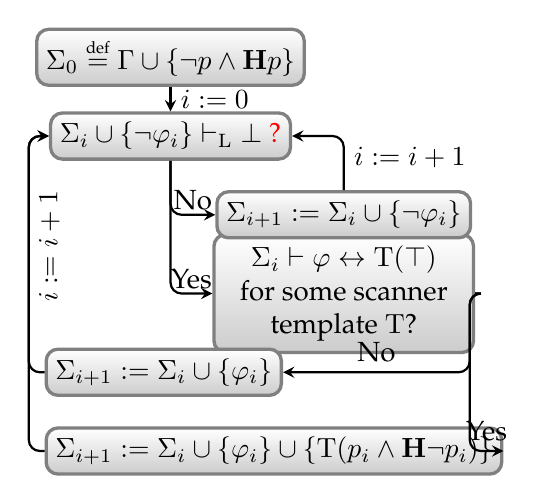
\begin{tikzpicture}[scale=1,>=stealth,
allapot/.style={ rectangle,minimum size=3mm,rounded corners=1.5mm,very thick,draw=black!50,top color=white,bottom color=black!20,
}]
\node[allapot](0) at (0,0){$\Sigma_0 \overset{\scalebox{.6}{def}}{=} \Gamma \cup \{ \lnot p \land \mathbf H p \}$};
\node[allapot](test) at (0,-1){$\Sigma_i \cup \{\lnot \varphi_i\}\vdash_{\mathrm{L}}\bot$ \textcolor{red}{?}};
\node[allapot] (yes-case) at (2.2,-3) {\begin{tabular}c$\Sigma_i \vdash \varphi \leftrightarrow \mathrm T(\top)$ \\ for some scanner \\ template $\mathrm T$?\end{tabular}};
\node[allapot] (no-case) at (2.2,-2) {$\Sigma_{i+1} := \Sigma_i\cup \{ \lnot \varphi_i\}$};
\node[allapot, anchor=west] (2ndYes) at (-1.6,-5) {$\Sigma_{i+1} := \Sigma_i \cup \{ \varphi_i\} \cup \{ \mathrm{T}(p_i\land \mathbf H \lnot p_i)\}$};
\node[allapot, anchor=west] (2ndNo) at (-1.6,-4) {$\Sigma_{i+1} := \Sigma_i \cup \{ \varphi_i\}$};
\coordinate(csatl) at (-1.8,-3) {} {};
\coordinate(csatl2) at (3.8,-3.6) {};
\begin{scope}[->, thick, rounded corners=4pt]
 \draw (0)--(test) node[midway, right]{$i:=0$};
 \draw (test)|-(no-case) node[pos=.75, above, inner sep=.5mm]{No};
 \draw (test)|-(yes-case)node[pos=.75, above, inner sep=.5mm]{Yes};
 \draw (yes-case)-|(csatl2)|-(2ndNo) node[pos=.75, above]{No};
 \draw (yes-case)-|(csatl2)|-(2ndYes) node[pos=.75, above]{Yes};
 \draw (2ndNo)-|(csatl)|-(test) node[pos=0.15, below, rotate=90]{$i:=i+1$};
 \draw (2ndYes)-|(csatl)|-(test);
 \draw (no-case)|-(test) node[pos=.3, right]{$i:=i+1$};
\end{scope}
\end{tikzpicture}\]
\end{minipage}

\end{frame}


\szakasz[Irr. can. submodel]{Irreflexive canonical submodel}

\begin{frame}
\frametitle{Canonical Kamp model}

\[\mathfrak M_{\mathbf O} \defegy \left( W_{\mathbf O}, <_{\mathbf O}, \equiv_{\mathbf O}, V_{\mathbf O}\right)   \]
where
\begin{itemize}
\item $W_{\mathbf O} \defegy \{\Gamma \, :\, \textup{$ \Gamma$  is a maximally $\mathbf O$-consistent \cemph{IRR-theory}} \}$,
\item $\Gamma <_{\mathbf O}\Gamma'$ iff $\FB^-(\Gamma )\subseteq  \Gamma'$ \bemph{Remember that these are equivalent: 
\\ \hfill $\begin{tomb}{rcl}
          \FB^-(\Gamma )&\subseteq & \Gamma'
\\ \Gamma &\supseteq & \FD^+(\Gamma')
\\ \Gamma &\supseteq & \PB^-(\Gamma')
\\ \PD^+(\Gamma)&\subseteq & \Gamma'
\end{tomb}$}
\item $\Gamma \equiv_{\mathbf O}\Gamma'$ iff $\Box^-(\Gamma )\subseteq \Gamma'$, \bemph{Similarly:
$\begin{tomb}{rcl}
          \Box^-(\Gamma )&\subseteq & \Gamma'
\\ \Gamma &\supseteq & \Diamond^+(\Gamma')
\end{tomb}$}
\item $\Gamma \in V_{\mathbf O}(p) \defekv p\in \Gamma$.
\end{itemize}


\end{frame}

%%%%%%%%%%%%%%%%%%%%%%%%%%%%%%%%%%%%%%%%%%%%%%%%%%%%%%%%%%%%%%%%%%%%%%%%%%%%%%%%%%%%%%%%%%%%%%%%%%%5

\begin{frame}
\frametitle{The \cemph{old} Existence Lemmas}
Let $\mathrm L$ denote the dual pair of $\mathrm M$. The \cemph{new} Existence Lemmas:
\[\mathrm M \psi \in \Gamma  \mathrel{\cemph{\Longrightarrow}} \existsin {\Gamma'}{\cemph{W_\mathbf O}} \big[\Gamma' \supseteq \mathrm{L}^-(\Gamma) \textup{ and } \psi \in \Gamma' \big]\]

\hrule
\medskip

\magyi{The old proofs ensured the existence of a max. con. set, but now we need the existence of a max.con. \cemph{IRR-theory}!}

\bigskip

But we can reuse the proof to state the following lemma very useful lemma:

\bigskip

\dzsa{Lemma} If $\Gamma$ is a max.con. set, then 
\[ \mathrm M \varphi \in \Gamma \quad \Longrightarrow\quad \mathrm L^-(\Gamma) \cup\{\varphi\}\not \derives[O] \bot\]
\dzsa{proof}
\bemph{\tiny\[ \begin{tomb}{rcll}
   \mathrm L^- (\Gamma) \cup \{\varphi\}&\vdash_{\mathbf O}&\bot &\textup{indirect assumption}
\\ \mathrm L^- (\Gamma)&\vdash_{\mathbf O}& \lnot \varphi &\textup{Deduction theorem}
\\ \exists \chi_1,  \cdots,\chi_{n}&\vdash_{\mathbf O}& \lnot \varphi &\textup{def.of $\mathrm L^- (\Gamma)\vdash_{\mathbf O}$}
\\ &\vdash_{\mathbf O}& (\chi_1 \land \dots \land \chi_{n}) \lthen \lnot \varphi &\textup{def.of $(\chi_1 \land \dots \land \chi_{n})\vdash_{\mathbf O}$}
\\ &\vdash_{\mathbf O}& \mathrm L (\chi_1 \land \dots \land \chi_{n}) \lthen \mathrm L \lnot \varphi &\textup{Lemmon}
\\ &\vdash_{\mathbf O}& (\mathrm L \chi_1 \land \dots \land \mathrm L\chi_{n})\lthen \mathrm L \lnot \varphi &\textup{A-axiom}
\\ \mathrm L \chi_1, \cdots ,\mathrm L\chi_{n} &\vdash_{\mathbf O}& \mathrm L \lnot \varphi & \textup{def.of $(\mathrm L \chi_1 \land \dots \land \mathrm L \chi_{n})\vdash_{\mathbf O}$}
\\ \Gamma &\vdash_{\mathbf O}& \mathrm L \lnot \varphi &\chi\in \mathrm L^-(\Gamma) \Leftrightarrow \mathrm L \chi\in \Gamma
\\ \Gamma &\vdash_{\mathbf O}& \lnot \FD\varphi &\textup{Duality}
\\ \Gamma \cup \{ \FD\varphi \}&\vdash_{\mathbf O}& \bot &\textup{Deduction theorem}
\\ \Gamma &\vdash_{\mathbf O}& \bot &\textup{we assumed that $\FD \varphi \in \Gamma$}
\end{tomb}\]}

\end{frame}
%%%%%%%%%%%%%%%%%%%%%%%%%%%%%%%%%%%%%%%%% NEXT SLIDE %%%%%%%%%%%%%%%%%%%%%%%%%%%%%%%%%%%%%%%%555555
\begin{frame}
\frametitle{The \cemph{new} Existence Lemmas}
Let $\mathrm L$ denote the dual pair of $\mathrm M$.
\[\mathrm M \psi \in \Gamma  \mathrel{\cemph{\Longrightarrow}} \existsin {\Gamma'}{\cemph{W_\mathbf O}} \big[\Gamma' \supseteq \mathrm{L}^-(\Gamma) \textup{ and } \psi \in \Gamma' \big]\]

\hrule
\medskip

\magyi{The old proof ensured the existence of a max. con. set, but now we need the existence of a max.con. \cemph{IRR-theory}!}

\[ \begin{tomb}{rcll}
   \Gamma &\ni& \mathrm M \varphi &\textup{assumption}
\\ \Gamma &\ni& \mathrm M (\varphi\land \top) &
\\ \existsin p{\mathrm{At}}\; \Gamma &\ni& \mathrm M (\underbrace{\varphi \land p\land \PB \lnot p}_{\psi})  &\textup{$\Gamma$ is IRR ($\mathrm T= \FD \bigcirc$)}
\end{tomb}\]
Remember that this $p$ does not occur in $\varphi$! Now let $\psi\defegy \varphi \land p\land \PB \lnot p$. Then we have from our \bemph{old proof} that
$\Sigma_0\defegy \mathrm{L}^- (\Gamma) \cup \{\psi\}$ is $\mathbf O$-consistent.

\bigskip
\cemph{We cannot use the IRR version of Lindenbaum lemma since it is possible that \emph{only finitely many} atomic sentences do not occur in $\mathrm{L}^-(\Gamma)$.}
\bigskip

The point is, that we have to choose the desired $p$-s wisely, because they can occur $\mathrm{L}^-(\Gamma)$. In fact, If we start with $\mathrm L^-$, then the IRR property of $\Gamma$ will provide us a nice infinite set of suitable $p$-s.

%But we can modify the proof of this lemma in a way to provide the desired $\Gamma'$.
\end{frame}

%%%%%%%%%%%%%%%%%%%%%%%%%%%%%%%%%%%%%%%%%%%%%%%%%%%%%%%%%%%%%%%%%%%%%%%%%%%%%%%%%%%%%%%%%%%%%%%%%%%5

\begin{frame}[t]
	\frametitle{The new Existence Lemmas}
\scriptsize
\begin{minipage}{.5\textwidth}
It is clear by the construction that $\bigcup \{\Sigma_i: i\in \omega\}$ is consistent. Now we have to prove that it is an IRR theory. 

It is enough to show that in every step, at the Yes-Yes-case we can find a suitable $p_i$ (even if it occurs in $\Sigma_i$).

\begin{itemize}
\item<1-> If we are at the Yes-Yes case, $\Sigma_i \derives[O] \varphi_i $, i.e., $\Sigma_i \derives[O] \mathrm{T}(\top)$.
\item<2-> Using that we can show that  $\mathrm M(\psi \land \bigwedge(\Sigma_i-\Sigma_0)\land \varphi_i )\in \Gamma$:
\only<2>{\[ \begin{tomb}{rcll}
   \Gamma & \not \ni & \mathrm M(\psi \land \bigwedge(\Sigma_i-\Sigma_0)\land \varphi_i ) &\magyi{indirect assumption}
\\ \Gamma & \ni & \lnot \mathrm M(\psi \land \bigwedge(\Sigma_i-\Sigma_0)\land \varphi_i ) &\magyi{$\Gamma$ is max.con.}
\\ \Gamma & \ni & \mathrm L ((\psi \land \bigwedge(\Sigma_i-\Sigma_0))\lthen \lnot \varphi_i ) &\magyi{push in the $\lnot$}
\\ \Box^-(\Gamma) & \ni & (\psi \land \bigwedge(\Sigma_i-\Sigma_0))\lthen \lnot \varphi_i  &\magyi{def.of $\Box^-$}
\\ \Sigma_0 & \ni & (\psi \land \bigwedge(\Sigma_i-\Sigma_0))\lthen \lnot \varphi_i  &\magyi{$\Sigma_0\defegy \mathrm{L}^-(\Gamma) \cup \{\psi\}$}
\\ \Sigma_0 & \ni & \psi  &\magyi{$\Sigma_0\defegy \mathrm{L}^-(\Gamma) \cup \{\psi\}$}
\\ \Sigma_0 & \derives[O] & \bigwedge(\Sigma_i-\Sigma_0)\lthen \lnot \varphi_i  &\magyi{modus ponens}
\\ \Sigma_i & \derives[O] & \bigwedge(\Sigma_i-\Sigma_0)\lthen \lnot \varphi_i  &\magyi{$\Sigma_i\supseteq \Sigma_0$}
\\ \Sigma_i & \derives[O] & \bigwedge(\Sigma_i-\Sigma_0)  &\magyi{all conjuncts of $\bigwedge(\Sigma_i-\Sigma_0)$ are in $\Sigma_i$}
\\ \Sigma_i & \derives[O] & \lnot \varphi_i  &\magyi{modus ponens, contradiction}
\end{tomb} \]}
\item<3-> But $\mathrm M(\psi \land \bigwedge(\Sigma_i-\Sigma_0)\land \varphi_i )$, \\ i.e.,  
$\mathrm M(\psi \land \bigwedge(\Sigma_i-\Sigma_0)\land \mathrm{T}(\top) )$ is a scanner template.
\item<4-> Then since $\Gamma$ itself was IRR, there is a $p_i$ not in $\psi \land \bigwedge(\Sigma_i-\Sigma_0)$, s.t. $\mathrm M(\psi \land \bigwedge(\Sigma_i-\Sigma_0)\land \mathrm T(p_i\land \PB \lnot p_i) )\in \Gamma$.
\item<5-> \textcolor{white}{hely} \\ [-3ex]\mbox{Then we have that $\Box ^-(\Gamma) \cup \{\psi \land \bigwedge(\Sigma_i-\Sigma_0)\land \mathrm T(p_i\land \PB \lnot p_i)\}$ is consistent.}
\item<6-> \textcolor{white}{hely} \\ [-3ex]\mbox{Then we have that $\underbrace{\underbrace{\Box ^-(\Gamma) \cup \{\psi\}}_{\Sigma_0} \cup (\Sigma_i-\Sigma_0)}_{\Sigma_i}\cup\{\mathrm T(p_i\land \PB \lnot p_i)\} \textup{ is consistent.}$}
\end{itemize}
\end{minipage}
\quad
\begin{minipage}{.4\textwidth}
\vspace{-3cm}
\only<1,3->{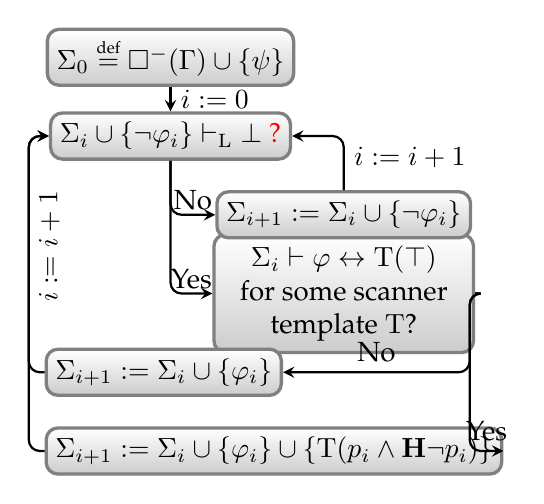
\begin{tikzpicture}[scale=1,>=stealth,
allapot/.style={ rectangle,minimum size=3mm,rounded corners=1.5mm,very thick,draw=black!50,top color=white,bottom color=black!20,
}]
\node[allapot](0) at (0,0){$\Sigma_0 \overset{\scalebox{.6}{def}}{=} \Box^-(\Gamma) \cup \{ \psi \}$};
\node[allapot](test) at (0,-1){$\Sigma_i \cup \{\lnot \varphi_i\}\vdash_{\mathrm{L}}\bot$ \textcolor{red}{?}};
\node[allapot] (yes-case) at (2.2,-3) {\begin{tabular}c$\Sigma_i \vdash \varphi \leftrightarrow \mathrm T(\top)$ \\ for some scanner \\ template $\mathrm T$?\end{tabular}};
\node[allapot] (no-case) at (2.2,-2) {$\Sigma_{i+1} := \Sigma_i\cup \{ \lnot \varphi_i\}$};
\node[allapot, anchor=west] (2ndYes) at (-1.6,-5) {$\Sigma_{i+1} := \Sigma_i \cup \{ \varphi_i\} \cup \{ \mathrm{T}(p_i\land \mathbf H \lnot p_i)\}$};
\node[allapot, anchor=west] (2ndNo) at (-1.6,-4) {$\Sigma_{i+1} := \Sigma_i \cup \{ \varphi_i\}$};
\coordinate(csatl) at (-1.8,-3) {} {};
\coordinate(csatl2) at (3.8,-3.6) {};
\begin{scope}[->, thick, rounded corners=4pt]
 \draw (0)--(test) node[midway, right]{$i:=0$};
 \draw (test)|-(no-case) node[pos=.75, above, inner sep=.5mm]{No};
 \draw (test)|-(yes-case)node[pos=.75, above, inner sep=.5mm]{Yes};
 \draw (yes-case)-|(csatl2)|-(2ndNo) node[pos=.75, above]{No};
 \draw (yes-case)-|(csatl2)|-(2ndYes) node[pos=.75, above]{Yes};
 \draw (2ndNo)-|(csatl)|-(test) node[pos=0.15, below, rotate=90]{$i:=i+1$};
 \draw (2ndYes)-|(csatl)|-(test);
 \draw (no-case)|-(test) node[pos=.3, right]{$i:=i+1$};
\end{scope}
\end{tikzpicture}}
\end{minipage}

\end{frame}
%%%%%%%%%%%%%%%%%%%%%%%%%%%%%%%%%%%%%%%%%%%%%%%%%%%%%%%%%%%%%%%%%%%%%%%%%%%%%%%%%%%%%%%%%%%%%%%%%%%%%%%%%%%


\begin{frame}
\frametitle{Summary}
\begin{itemize}
\item The Truth Lemma goes through by our new existence lemma.
\item $V_\mathbf{O}$ is a Kamp-valuation by the axiom of the unpreventability of past.
\[ (UPP)\qquad \varphi \lthen \Box \varphi \textup{ where $\FD$ does not occur in $\varphi$}\]
\item $<_{\mathbf O}$ is irreflexive by construction (all our canonical worlds are IRR theories).
\item $<_{\mathbf O}$ is transitive and non-branching by the canonicity of 4 and .3.
\item $\equiv_{\mathbf O}$ is reflexive, transitive and symmetric by the canonicity of T, 4 and B.
\item $\Gamma \equiv_{\mathbf O} \Delta \lthen \Gamma\not <_{\mathbf O}\Delta $ comes from (UPP) and from the construction:
There is a $p\land \PB \lnot p\in \Delta$, by UPP, $\Box (p\land \PB \lnot p)\in \Delta$, by def of $\equiv_{\mathbf O}$, and the symmetry of it, $p\land \PB \lnot p\in \Gamma$.
But $\Gamma <_{\mathbf O}\Delta$ would mean that $\PB^-(\Delta)\subseteq \Gamma$, so $\lnot p\in \Gamma$ which causes a contradiction.
\item $(w \equiv v \land w'<w ) \lthen \existsp {v'<v} \;w'\equiv v'$ -- We prove this on the next slide
\item $\forallp{w,v}\existsp{w'<w}\existsp {v'<v} \;w\equiv v$ As in usual, we can take the generated submodels to validate this.
\item \cemph{$\forallp{w,v} (w \equiv v \land w\neq v) \existsp{w'>w}\forallp {v'>v} \;w'\not\equiv v'$} that is not true, we will have to suffer with this later
\end{itemize}
\end{frame}


\item $x \equiv y \lthen x\not <y$ \bemph{}
\item $(w \equiv v \land w'<w ) \lthen \existsp {v'<v} \;w'\equiv v'$  \hfill  ``sharing the same past''
\item $\forallp{w,v}\existsp{w'<w}\existsp {v'<v} \;w\equiv v$ \hfill class common root
\item $\forallp{w,v} (w \equiv v \land w\neq v) \existsp{w'>w}\forallp {v'>v} \;w'\not\equiv v'$ \\ \hfill maximality of histories
\end{itemize}

\felirat{1}{1}{.7}{4.5}{3}{
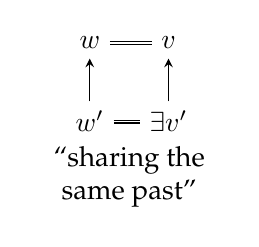
\begin{tikzpicture}[world/.style={inner sep=.4mm, fill=black, circle},>=stealth, scale=1]
\node (v1) at (0,0) {$w'$};
\node (v2) at (0,1) {$w$};
\node (v3) at (1,0) {$\exists v'$};
\node (v4) at (1,1) {$v$};
\draw[->]  (v1) -- (v2);
\draw[->]  (v3) -- (v4);
\draw[double]  (v1) -- (v3);
\draw[double]  (v2) -- (v4);
\node at (0.5,-0.7) {\begin{tabular}{c}``sharing the \\same past''\end{tabular}};
\end{tikzpicture}}
\felirat{1}{1}{.7}{4.5}{1.125}{
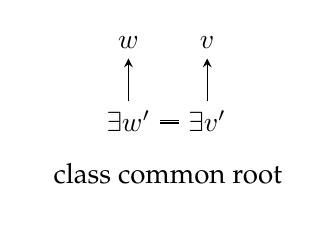
\begin{tikzpicture}[world/.style={inner sep=.4mm, fill=black, circle},>=stealth, scale=1]
\node (v1) at (0,0) {$\exists w'$};
\node (v2) at (0,1) {$w$};
\node (v3) at (1,0) {$\exists v'$};
\node (v4) at (1,1) {$v$};
\draw[->]  (v1) -- (v2);
\draw[->]  (v3) -- (v4);
\draw[double]  (v1) -- (v3);
%\draw[double]  (v2) -- (v4);
\node at (0.5,-0.7) {\begin{tabular}{c}class common root\end{tabular}};
\end{tikzpicture}}
\felirat{1}{1}{.7}{4.5}{-.75}{
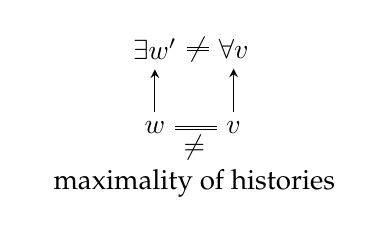
\begin{tikzpicture}[world/.style={inner sep=.4mm, fill=black, circle},>=stealth, scale=1]
\node at (0.5,-0.25) {$\neq$};
\node (v1) at (0,0) {$w$};
\node (v2) at (0,1) {$\exists w'$};
\node (v3) at (1,0) {$v$};
\draw[->]  (v1) -- (v2);
\draw[double]  (v1) -- (v3);
%\pause %%%%%%%%%%%%%%%%%% --- PAUSE --- %%%%%%%%%%%%%%%%%%
\node (v4) at (1,1) {$\forall v$};
\draw[double]  (v2) -- (v4);
\draw[->]  (v3) -- (v4);
\node at (0.5,-0.7) {\begin{tabular}{c}maximality of histories\end{tabular}};
\node at (0.5,1) {$\!\!\!\not$};
\end{tikzpicture}}
\pause

\end{minipage}}

\end{frame}


%%%%%%%%%%%%%%%%%%%%%%%%%%%%%%%%%%%%%%%%%%%%%%%%%%%%%%%%%%%%%%%%%%%%%%%%%%%%%%%%%%%%%%%%%%%%%%%%%%%5

\end{document}

